% Options for packages loaded elsewhere
\PassOptionsToPackage{unicode}{hyperref}
\PassOptionsToPackage{hyphens}{url}
%
\documentclass[
  ignorenonframetext,
  aspectratio=169,
  russian,
]{beamer}
\usepackage{pgfpages}
\setbeamertemplate{caption}[numbered]
\setbeamertemplate{caption label separator}{: }
\setbeamercolor{caption name}{fg=normal text.fg}
\beamertemplatenavigationsymbolshorizontal
% Prevent slide breaks in the middle of a paragraph
\widowpenalties 1 10000
\raggedbottom
\setbeamertemplate{part page}{
  \centering
  \begin{beamercolorbox}[sep=16pt,center]{part title}
    \usebeamerfont{part title}\insertpart\par
  \end{beamercolorbox}
}
\setbeamertemplate{section page}{
  \centering
  \begin{beamercolorbox}[sep=12pt,center]{section title}
    \usebeamerfont{section title}\insertsection\par
  \end{beamercolorbox}
}
\setbeamertemplate{subsection page}{
  \centering
  \begin{beamercolorbox}[sep=8pt,center]{subsection title}
    \usebeamerfont{subsection title}\insertsubsection\par
  \end{beamercolorbox}
}
\AtBeginPart{
  \frame{\partpage}
}
\AtBeginSection{
  \ifbibliography
  \else
    \frame{\sectionpage}
  \fi
}
\AtBeginSubsection{
  \frame{\subsectionpage}
}

\usepackage{amsmath,amssymb}
\usepackage{iftex}
\ifPDFTeX
  \usepackage[T1]{fontenc}
  \usepackage[utf8]{inputenc}
  \usepackage{textcomp} % provide euro and other symbols
\else % if luatex or xetex
  \usepackage{unicode-math}
  \defaultfontfeatures{Scale=MatchLowercase}
  \defaultfontfeatures[\rmfamily]{Ligatures=TeX,Scale=1}
\fi
\usepackage{lmodern}
\usetheme[]{metropolis}
\ifPDFTeX\else  
    % xetex/luatex font selection
\fi
% Use upquote if available, for straight quotes in verbatim environments
\IfFileExists{upquote.sty}{\usepackage{upquote}}{}
\IfFileExists{microtype.sty}{% use microtype if available
  \usepackage[]{microtype}
  \UseMicrotypeSet[protrusion]{basicmath} % disable protrusion for tt fonts
}{}
\usepackage{xcolor}
\newif\ifbibliography
\setlength{\emergencystretch}{3em} % prevent overfull lines
\setcounter{secnumdepth}{-\maxdimen} % remove section numbering


\providecommand{\tightlist}{%
  \setlength{\itemsep}{0pt}\setlength{\parskip}{0pt}}\usepackage{longtable,booktabs,array}
\usepackage{calc} % for calculating minipage widths
\usepackage{caption}
% Make caption package work with longtable
\makeatletter
\def\fnum@table{\tablename~\thetable}
\makeatother
\usepackage{graphicx}
\makeatletter
\newsavebox\pandoc@box
\newcommand*\pandocbounded[1]{% scales image to fit in text height/width
  \sbox\pandoc@box{#1}%
  \Gscale@div\@tempa{\textheight}{\dimexpr\ht\pandoc@box+\dp\pandoc@box\relax}%
  \Gscale@div\@tempb{\linewidth}{\wd\pandoc@box}%
  \ifdim\@tempb\p@<\@tempa\p@\let\@tempa\@tempb\fi% select the smaller of both
  \ifdim\@tempa\p@<\p@\scalebox{\@tempa}{\usebox\pandoc@box}%
  \else\usebox{\pandoc@box}%
  \fi%
}
% Set default figure placement to htbp
\def\fps@figure{htbp}
\makeatother

\IfFileExists{plex-otf.sty}{
  %% Full TeXlive
  % \usepackage[%
  %   % math,
  %   RM={Scale=0.94},SS={Scale=0.94},SScon={Scale=0.94},TT={Scale=MatchLowercase,FakeStretch=0.9},DefaultFeatures={Ligatures=Common}
  % ]{plex-otf}
}{
  %% TinyTeX
  \usepackage{libertine}
}

%%% Load theme
% https://deic.uab.cat/~iblanes/beamer_gallery/
\IfFileExists{beamerthemegotham.sty}{
  %% Full TeXlive
  \usetheme{gotham}
  \gothamset{
    numbering=totalpagenumber,
    parttocframe default=off,
    sectiontocframe default=off,
    subsectiontocframe default=off,
  }
}{
  %% TinyTeX
  \usetheme{Madrid}
}
\metroset{progressbar=frametitle,sectionpage=progressbar,numbering=fraction}
\makeatletter
\@ifpackageloaded{caption}{}{\usepackage{caption}}
\AtBeginDocument{%
\ifdefined\contentsname
  \renewcommand*\contentsname{Содержание}
\else
  \newcommand\contentsname{Содержание}
\fi
\ifdefined\listfigurename
  \renewcommand*\listfigurename{Список иллюстраций}
\else
  \newcommand\listfigurename{Список иллюстраций}
\fi
\ifdefined\listtablename
  \renewcommand*\listtablename{Список таблиц}
\else
  \newcommand\listtablename{Список таблиц}
\fi
\ifdefined\figurename
  \renewcommand*\figurename{Рисунок}
\else
  \newcommand\figurename{Рисунок}
\fi
\ifdefined\tablename
  \renewcommand*\tablename{Таблица}
\else
  \newcommand\tablename{Таблица}
\fi
}
\@ifpackageloaded{float}{}{\usepackage{float}}
\floatstyle{ruled}
\@ifundefined{c@chapter}{\newfloat{codelisting}{h}{lop}}{\newfloat{codelisting}{h}{lop}[chapter]}
\floatname{codelisting}{Список}
\newcommand*\listoflistings{\listof{codelisting}{Листинги}}
\makeatother
\makeatletter
\makeatother
\makeatletter
\@ifpackageloaded{caption}{}{\usepackage{caption}}
\@ifpackageloaded{subcaption}{}{\usepackage{subcaption}}
\makeatother

\ifLuaTeX
\usepackage[bidi=basic]{babel}
\else
\usepackage[bidi=default]{babel}
\fi
\babelprovide[main,import]{russian}
\babelprovide[import]{english}
% get rid of language-specific shorthands (see #6817):
\let\LanguageShortHands\languageshorthands
\def\languageshorthands#1{}
\usepackage{csquotes}
\usepackage{bookmark}

\IfFileExists{xurl.sty}{\usepackage{xurl}}{} % add URL line breaks if available
\urlstyle{same} % disable monospaced font for URLs
\hypersetup{
  pdftitle={Презентация по лабораторной работе №2},
  pdfauthor={Маркеш В.Н.Грасимилде.},
  pdflang={ru-RU},
  hidelinks,
  pdfcreator={LaTeX via pandoc}}


\title{Презентация по лабораторной работе №2}
\subtitle{Архитектура компьютеров и Операционные Системы}
\author{Маркеш В.Н.Грасимилде.}
\date{Invalid Date}
\institute{Российский университет дружбы народов, Москва, Россия}

\begin{document}
\frame{\titlepage}


\section{Цель
работы}\label{ux446ux435ux43bux44c-ux440ux430ux431ux43eux442ux44b}

\begin{frame}{Цель работы}
Изучение идеалогии, применение средств контроля версий и освоение умения
по работе с git.
\end{frame}

\section{Задание}\label{ux437ux430ux434ux430ux43dux438ux435}

\begin{frame}{Задание}
\begin{itemize}[<+->]
\tightlist
\item
  Создать базовую конфигурацию для работы с git.
\item
  Создать ключ SSH.
\item
  Создать ключ PGP.
\item
  Настроить подписи git.
\item
  Зарегистрироваться на Github.
\item
  Создать локальный каталог для выполнения заданий по предмету.
\end{itemize}
\end{frame}

\begin{frame}{Создание базовой конфигурации для работы с git.}
\phantomsection\label{ux441ux43eux437ux434ux430ux43dux438ux435-ux431ux430ux437ux43eux432ux43eux439-ux43aux43eux43dux444ux438ux433ux443ux440ux430ux446ux438ux438-ux434ux43bux44f-ux440ux430ux431ux43eux442ux44b-ux441-git.}
Установление git и gh:

\begin{figure}

{\centering 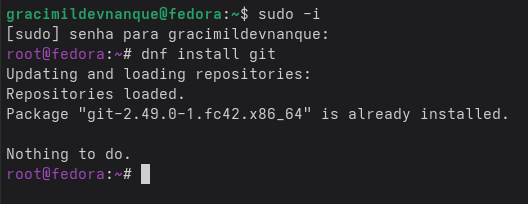
\includegraphics[width=0.7\linewidth,height=\textheight,keepaspectratio]{./image/1.PNG}

}

\caption{Установление git}

\end{figure}%%
\begin{figure}

{\centering 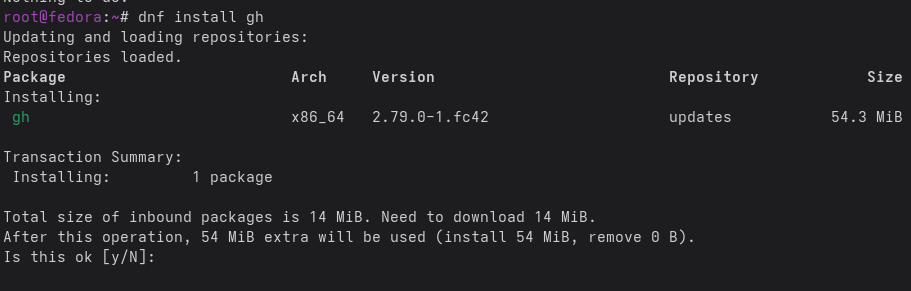
\includegraphics[width=0.7\linewidth,height=\textheight,keepaspectratio]{./image/2.PNG}

}

\caption{Установление gh}

\end{figure}%
\end{frame}

\begin{frame}{Создание базовой конфигурации для работы с git.}
\phantomsection\label{ux441ux43eux437ux434ux430ux43dux438ux435-ux431ux430ux437ux43eux432ux43eux439-ux43aux43eux43dux444ux438ux433ux443ux440ux430ux446ux438ux438-ux434ux43bux44f-ux440ux430ux431ux43eux442ux44b-ux441-git.-1}
В качестве имя и email владельца репозитории задаю свои имя и email и
настраиваю utf-8:

\begin{figure}

{\centering 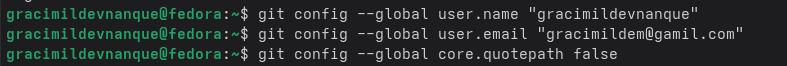
\includegraphics[width=0.7\linewidth,height=\textheight,keepaspectratio]{./image/3.PNG}

}

\caption{имя и email владельца}

\end{figure}%
\end{frame}

\begin{frame}{Создание базовой конфигурации для работы с git.}
\phantomsection\label{ux441ux43eux437ux434ux430ux43dux438ux435-ux431ux430ux437ux43eux432ux43eux439-ux43aux43eux43dux444ux438ux433ux443ux440ux430ux446ux438ux438-ux434ux43bux44f-ux440ux430ux431ux43eux442ux44b-ux441-git.-2}
Задаю имя начальной ветки и паррамеры autocrlf и safecrlf:

\begin{figure}

{\centering 
\includegraphics[width=0.7\linewidth,height=\textheight,keepaspectratio]{./image/4.PNG}

}

\caption{имя начальной ветки и паррамеры}

\end{figure}%
\end{frame}

\begin{frame}{Создание ключ ssh}
\phantomsection\label{ux441ux43eux437ux434ux430ux43dux438ux435-ux43aux43bux44eux447-ssh}
Создаю ключи ssh по алгоритму rsa с размером 4096 бит:

\begin{figure}

{\centering 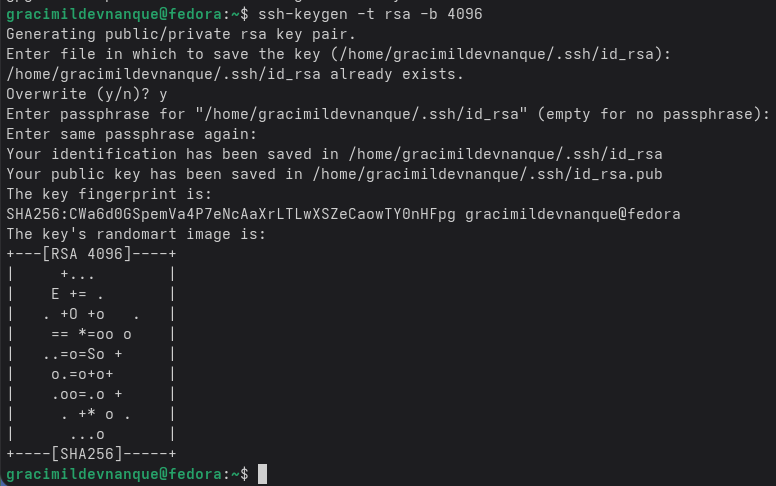
\includegraphics[width=0.7\linewidth,height=\textheight,keepaspectratio]{./image/5.PNG}

}

\caption{Создание ключ ssh}

\end{figure}%
\end{frame}

\begin{frame}{Создание ключ gpg}
\phantomsection\label{ux441ux43eux437ux434ux430ux43dux438ux435-ux43aux43bux44eux447-gpg}
Генерирую ключ gpg --full-generate-key:

\begin{figure}

{\centering 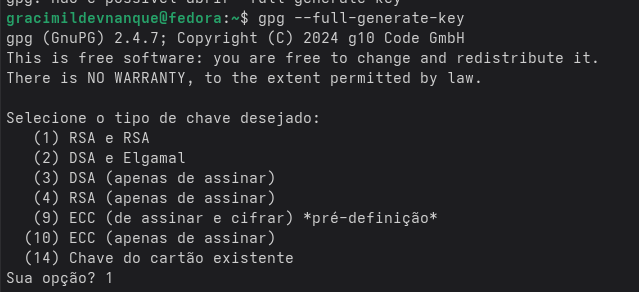
\includegraphics[width=0.7\linewidth,height=\textheight,keepaspectratio]{./image/6.PNG}

}

\caption{Создание ключ gpg}

\end{figure}%
\end{frame}

\begin{frame}{Создание ключ gpg}
\phantomsection\label{ux441ux43eux437ux434ux430ux43dux438ux435-ux43aux43bux44eux447-gpg-1}
Из предложенных опций выбираю тип RSA and RSA; размер 4096; срок
действия 0:

\begin{figure}

{\centering 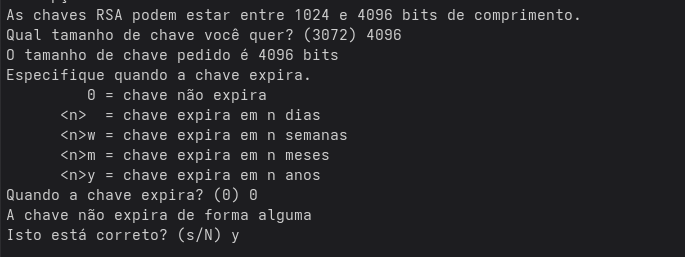
\includegraphics[width=0.7\linewidth,height=\textheight,keepaspectratio]{./image/7.PNG}

}

\caption{Настройки ключ gpg}

\end{figure}%
\end{frame}

\begin{frame}{Создание ключ gpg}
\phantomsection\label{ux441ux43eux437ux434ux430ux43dux438ux435-ux43aux43bux44eux447-gpg-2}
GPG запросил личную информацию, которая сохранится в ключе Имя и адрес
электронной почты:

\begin{figure}

{\centering 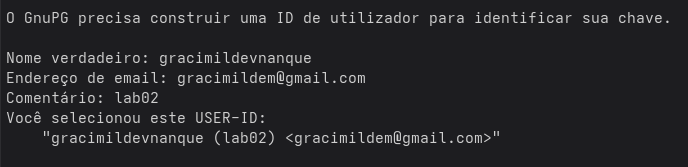
\includegraphics[width=0.7\linewidth,height=\textheight,keepaspectratio]{./image/8.PNG}

}

\caption{личная информация}

\end{figure}%
\end{frame}

\begin{frame}{Создание ключ gpg}
\phantomsection\label{ux441ux43eux437ux434ux430ux43dux438ux435-ux43aux43bux44eux447-gpg-3}
Вывожу список ключей:

\begin{figure}

{\centering 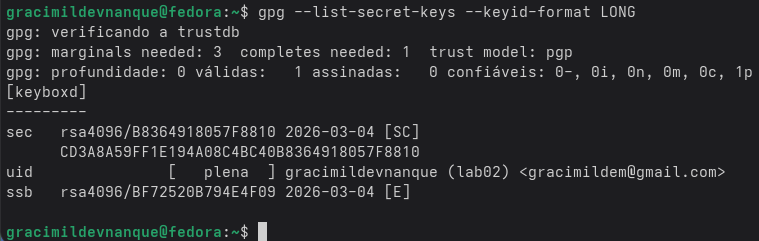
\includegraphics[width=0.7\linewidth,height=\textheight,keepaspectratio]{./image/10.PNG}

}

\caption{список ключей}

\end{figure}%
\end{frame}

\begin{frame}{Создание ключ gpg}
\phantomsection\label{ux441ux43eux437ux434ux430ux43dux438ux435-ux43aux43bux44eux447-gpg-4}
Установливаю xclip:

\begin{figure}

{\centering 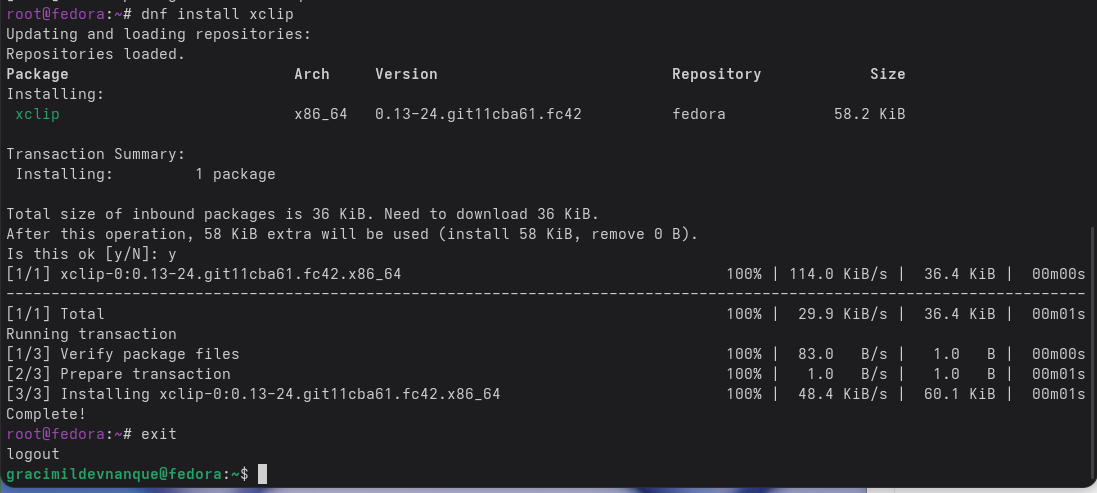
\includegraphics[width=0.7\linewidth,height=\textheight,keepaspectratio]{./image/11.PNG}

}

\caption{Установление xclip}

\end{figure}%
\end{frame}

\begin{frame}{Создание ключ gpg}
\phantomsection\label{ux441ux43eux437ux434ux430ux43dux438ux435-ux43aux43bux44eux447-gpg-5}
Cкопирую сгенерированный gpg ключ в буфер обмена:

\begin{figure}

{\centering 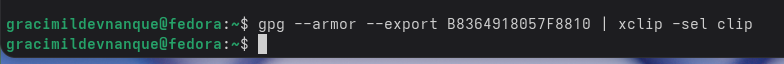
\includegraphics[width=0.7\linewidth,height=\textheight,keepaspectratio]{./image/13.PNG}

}

\caption{Копирование ключ gpg}

\end{figure}%
\end{frame}

\begin{frame}{Создание ключ gpg}
\phantomsection\label{ux441ux43eux437ux434ux430ux43dux438ux435-ux43aux43bux44eux447-gpg-6}
Далее перехожу в настройки GitHub, нажимаю на кнопку New GPG key и
вставляю полученный ключ:

\begin{figure}

{\centering 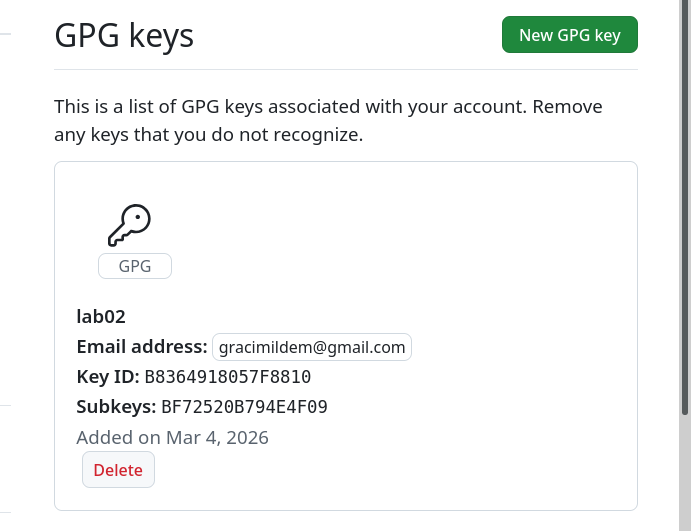
\includegraphics[width=0.7\linewidth,height=\textheight,keepaspectratio]{./image/14.PNG}

}

\caption{Добавлен ключ gpg}

\end{figure}%
\end{frame}

\begin{frame}{Создание ключ gpg}
\phantomsection\label{ux441ux43eux437ux434ux430ux43dux438ux435-ux43aux43bux44eux447-gpg-7}
Используя введёный email, указиваю Git применять его при подписи
коммитов:

\begin{figure}

{\centering 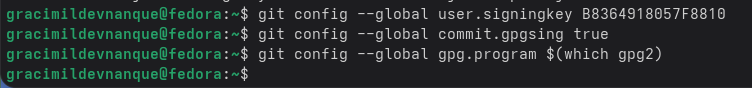
\includegraphics[width=0.7\linewidth,height=\textheight,keepaspectratio]{./image/15.PNG}

}

\caption{указиваю Git}

\end{figure}%
\end{frame}

\begin{frame}{Создание ключ gpg}
\phantomsection\label{ux441ux43eux437ux434ux430ux43dux438ux435-ux43aux43bux44eux447-gpg-8}
Начинаю авторизацию в gh используя gh auth login:

\begin{figure}

{\centering 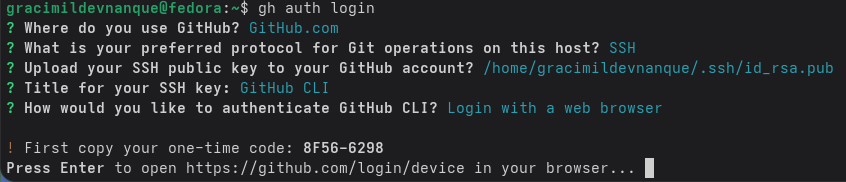
\includegraphics[width=0.7\linewidth,height=\textheight,keepaspectratio]{./image/16.PNG}

}

\caption{авторизацию в gh}

\end{figure}%
\end{frame}

\begin{frame}{Создание ключ gpg}
\phantomsection\label{ux441ux43eux437ux434ux430ux43dux438ux435-ux43aux43bux44eux447-gpg-9}
Завершаю авторизацию на броузер:

\begin{figure}

{\centering 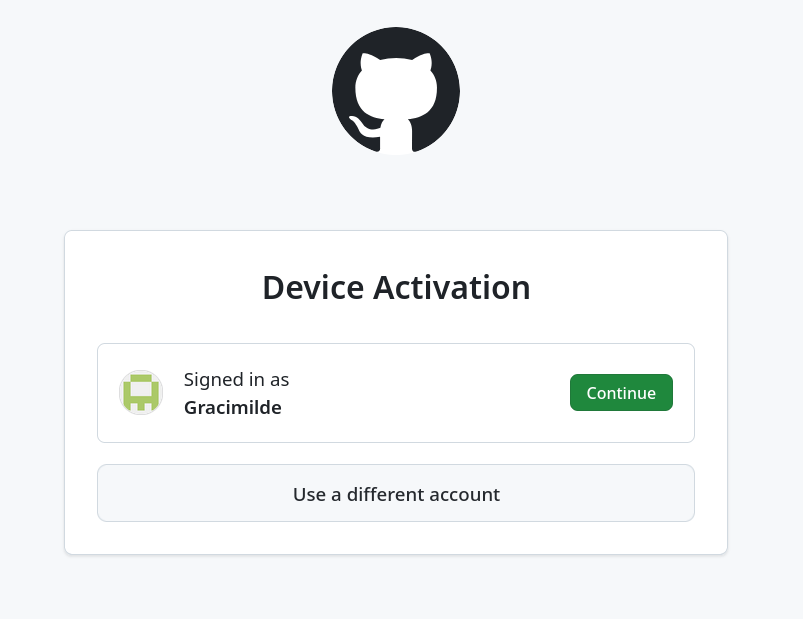
\includegraphics[width=0.7\linewidth,height=\textheight,keepaspectratio]{./image/17.PNG}

}

\caption{Авторизоваться через броузер.}

\end{figure}%
\end{frame}

\begin{frame}{Создание локального каталога для выполнения заданий.}
\phantomsection\label{ux441ux43eux437ux434ux430ux43dux438ux435-ux43bux43eux43aux430ux43bux44cux43dux43eux433ux43e-ux43aux430ux442ux430ux43bux43eux433ux430-ux434ux43bux44f-ux432ux44bux43fux43eux43bux43dux435ux43dux438ux44f-ux437ux430ux434ux430ux43dux438ux439.}
Создаю каталог \enquote{mkdir -p
\textasciitilde/work/study/2025-2026/}Операционные системы'':

\begin{figure}

{\centering 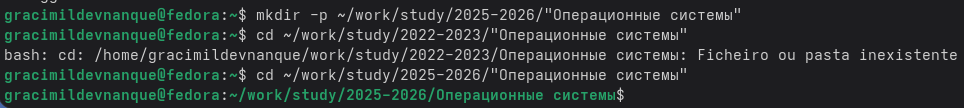
\includegraphics[width=0.7\linewidth,height=\textheight,keepaspectratio]{./image/19.PNG}

}

\caption{Создание каталог}

\end{figure}%
\end{frame}

\begin{frame}{Создание локального каталога для выполнения заданий.}
\phantomsection\label{ux441ux43eux437ux434ux430ux43dux438ux435-ux43bux43eux43aux430ux43bux44cux43dux43eux433ux43e-ux43aux430ux442ux430ux43bux43eux433ux430-ux434ux43bux44f-ux432ux44bux43fux43eux43bux43dux435ux43dux438ux44f-ux437ux430ux434ux430ux43dux438ux439.-1}
\begin{figure}

{\centering 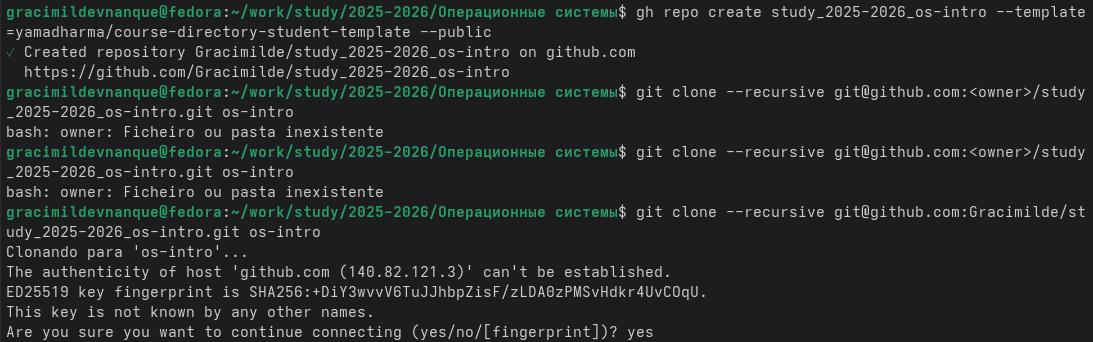
\includegraphics[width=0.7\linewidth,height=\textheight,keepaspectratio]{./image/20.PNG}

}

\caption{Создание каталог}

\end{figure}%
\end{frame}

\begin{frame}{Создание локального каталога для выполнения заданий.}
\phantomsection\label{ux441ux43eux437ux434ux430ux43dux438ux435-ux43bux43eux43aux430ux43bux44cux43dux43eux433ux43e-ux43aux430ux442ux430ux43bux43eux433ux430-ux434ux43bux44f-ux432ux44bux43fux43eux43bux43dux435ux43dux438ux44f-ux437ux430ux434ux430ux43dux438ux439.-2}
Удаляю лишные файлы:

\begin{figure}

{\centering 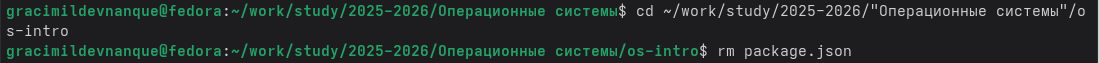
\includegraphics[width=0.7\linewidth,height=\textheight,keepaspectratio]{./image/21.PNG}

}

\caption{Удаление файла}

\end{figure}%
\end{frame}

\begin{frame}{Создание локального каталога для выполнения заданий.}
\phantomsection\label{ux441ux43eux437ux434ux430ux43dux438ux435-ux43bux43eux43aux430ux43bux44cux43dux43eux433ux43e-ux43aux430ux442ux430ux43bux43eux433ux430-ux434ux43bux44f-ux432ux44bux43fux43eux43bux43dux435ux43dux438ux44f-ux437ux430ux434ux430ux43dux438ux439.-3}
Создаю еще необходимые каталоги:

\begin{figure}

{\centering 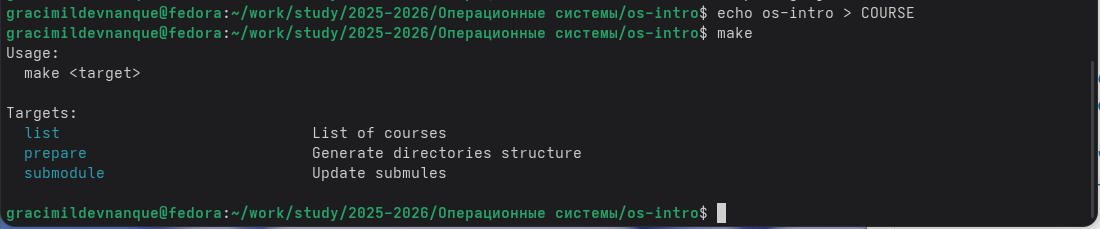
\includegraphics[width=0.7\linewidth,height=\textheight,keepaspectratio]{./image/22.PNG}

}

\caption{Создание необходимых каталогов}

\end{figure}%
\end{frame}

\begin{frame}{Создание локального каталога для выполнения заданий.}
\phantomsection\label{ux441ux43eux437ux434ux430ux43dux438ux435-ux43bux43eux43aux430ux43bux44cux43dux43eux433ux43e-ux43aux430ux442ux430ux43bux43eux433ux430-ux434ux43bux44f-ux432ux44bux43fux43eux43bux43dux435ux43dux438ux44f-ux437ux430ux434ux430ux43dux438ux439.-4}
Отправляю Файлы на сервер:

\begin{figure}

{\centering 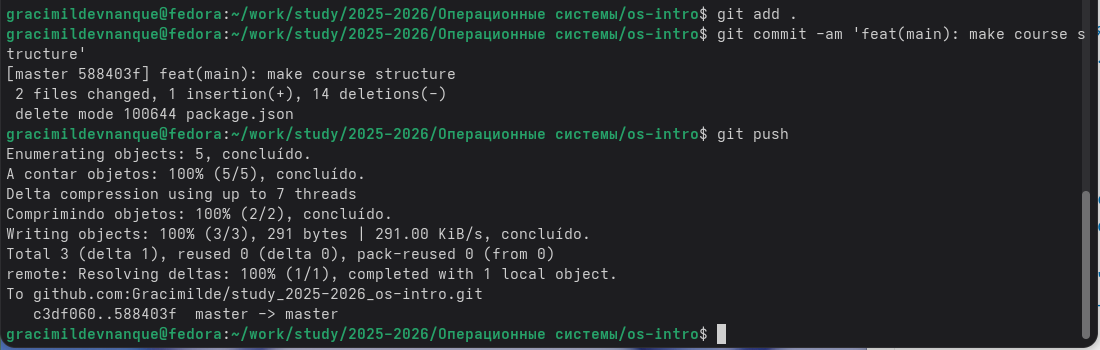
\includegraphics[width=0.7\linewidth,height=\textheight,keepaspectratio]{./image/23.PNG}

}

\caption{Отправление файлы на сервер}

\end{figure}%
\end{frame}

\section{Выводы}\label{ux432ux44bux432ux43eux434ux44b}

\begin{frame}{Выводы}
При выполнении лабораторной работы я изучила идеалогию, применение
средств контроля версий и освоеила умение по работе с git.
\end{frame}




\end{document}
